\documentclass[10pt, hyperref={colorlinks = true,linkcolor = blue}]{beamer}

\usetheme[progressbar=frametitle]{metropolis}
\usepackage{appendixnumberbeamer}
\usepackage{bm}
\usepackage{booktabs}
\usepackage[scale=2]{ccicons}
\usepackage{listings}
\lstset{
    language=R,
    basicstyle=\footnotesize\ttfamily,
    numbers=left,
    numberstyle=\tiny,
    stepnumber=1,
    numbersep=5pt,
    backgroundcolor=\color{white},
    showspaces=false,
    showstringspaces=false,
    showtabs=false,
    frame=single,
    tabsize=2,
    captionpos=b,
    breaklines=true,
    breakatwhitespace=false,
    title=\lstname,
    escapeinside={},
    keywordstyle=\color{blue},
    commentstyle=\color{green!40!black},
    morekeywords={install.packages, library, ggplot, geom\_bar, aes, ggtitle},
}


\usepackage{pgfplots}
\usepgfplotslibrary{dateplot}

\usepackage{xspace}
\newcommand{\themename}{\textbf{\textsc{metropolis}}\xspace}

\title{Introduction to Neural Networks}
\subtitle{Inspired from Prof. Xiangliang Zhang (KAUST) }
% \date{\today}
\date{}
\author{by Rishikesh Yadav (Postdoctoral Research Fellow)}
\institute{HEC Montr\'eal, McGill University, Canada}
% \titlegraphic{\hfill\includegraphics[height=1.5cm]{logo.pdf}}


\setbeamertemplate{caption}{\raggedright\insertcaption\par}

\begin{document}

\maketitle

\begin{frame}{Table of contents}
  \setbeamertemplate{section in toc}[sections numbered]
  \tableofcontents%[hideallsubsections]
\end{frame}



\begin{frame}[fragile]{References}
%	\setbeamercovered{transparent}
 %\begin{itemize}[<+->]
        \begin{itemize}
        \item Christopher M. Bishop (2007).
Pattern Recognition and Machine Learning
            \item Chollet, F., \& Allaire, J. J. (2018). \emph{Deep Learning with R}.
            \item There are some really good \href{https://www.coursera.org/}{Coursera courses} for deep learning, particularly with Python.
        \end{itemize}
\end{frame}

\begin{frame}{Goal}
\begin{itemize}
    \item The objectives of this short-course are:
    \begin{itemize}
    \item Understanding and learning regression using gradient descent algorithm 
        \item Understand the basics of deep learning and neural networks.
        \item Build and train simple feed-forward prediction and regression models using the R interface to Keras.
        \item Perform conditional density estimation using neural networks.
    \end{itemize}
\end{itemize}

\end{frame}

{\section{Background}
{\subsection{Linear Regression}
%\begin{frame}{Linear Regression}
%\begin{itemize}
%\item \textbf{Linear Regression} is a statistical method for modeling the relationship between a dependent variable and one or more independent variables.
%\item The relationship is modeled using a linear predictor function whose unknown parameters are estimated from the data.
%\[
%y = w_0 + w_1 x + \epsilon.
%\]
%\end{itemize}
%\end{frame}

\begin{frame}{Linear Regression (1) }
\setbeamercovered{transparent}
 \begin{itemize}[<+->]
    \item \textbf{Linear Regression} is a statistical method for modeling the relationship between a dependent variable and one or more independent variables.
    \item The relationship is modeled using a linear predictor function whose unknown parameters are estimated from the data.
    \item In its simplest form, with one dependent variable \(y\) and one independent variable \(x\), the linear regression model is:
    \[
    y = w_0 + w_1 x + \epsilon.
    \]
    where:
    \begin{itemize}
        \item \(y\) is the dependent variable (response variable).
        \item \(x\) is the independent variable (predictor variable).
        \item \(w_0\) is the intercept term, which represents the expected value of \(y\) when \(x = 0\).
        \item \(w_1\) is the slope term, which represents the change in \(y\) for a one-unit change in \(x\).
        \item \(\epsilon\) is the error term, which accounts for the variability in \(y\) that cannot be explained by the linear relationship with \(x\).
    \end{itemize}
    \end{itemize}
\end{frame}


\begin{frame}{Linear Regression (2) }
\setbeamercovered{transparent}
 \begin{itemize}[<+->]
  \item The parameters \(w_0\) and \(w_1\) are estimated from the data using methods such as \textbf{Ordinary Least Squares (OLS)}, which minimizes the sum of the squared differences between the observed values and the predicted values.
    \item The \textbf{OLS} estimate of the parameters can be obtained by solving the following normal equations:
    \[
    \begin{pmatrix}
    \hat{w}_0 \\
    \hat{w}_1
    \end{pmatrix}
    =
    \left( X^T X \right)^{-1} X^T y.
    \]
    where:
    \begin{itemize}
        \item \(X\) is the design matrix, including a column of ones for the intercept and a column of the predictor variable values.
        \item \(y\) is the vector of observed values of the dependent variable.
    \end{itemize}
    \item Linear regression can be extended to include multiple independent variables, resulting in \textbf{Multiple Linear Regression}:
    \[
    y = w_0 + w_1 x_1 + w_2 x_2 + \cdots + w_p x_p + \epsilon.
    \]
    where \(x_1, x_2, \ldots, x_p\) are the predictor variables.
\end{itemize}
\end{frame}

}

{\subsection{Gradient Descent Algorithm}

\begin{frame}{Gradient Descent Algorithm (1)}
\textbf{Gradient Descent Algorithm} is an optimization technique used to minimize a loss function by iteratively moving towards the minimum of the function.


  The main components of the gradient descent algorithm are:
\setbeamercovered{transparent}
 \begin{itemize}[<+->]
    \item \textbf{Loss Function}:
    \begin{itemize}
        \item The loss function measures the error or difference between the predicted values and the actual values. That means it measures how well the model's predictions match the actual data.
        \item The goal of gradient descent is to minimize this loss function to improve the accuracy of the model.
        \item Examples of loss functions include \textbf{Mean Squared Error (MSE)} for regression problems and \textbf{Cross-Entropy Loss} for classification problems.
        \item Mathematically, for a set of predictions \(\hat{y}\) and actual values \(y\), the Mean Squared Error is given by:
        \[
        \text{MSE} = \frac{1}{n} \sum_{i=1}^{n} (y_i - \hat{y}_i)^2.
        \]
\end{itemize}
      \end{itemize}
 \end{frame}
 
 \begin{frame}{Gradient Descent Algorithm (2)}
 \setbeamercovered{transparent}
 \begin{itemize}[<+->]
  \item \textbf{Gradient}:
    \begin{itemize}
        \item The gradient is a vector of partial derivatives of the loss function with respect to all the parameters of the model.
        \item It points in the direction of the steepest ascent of the function.
        \item In gradient descent, we move in the opposite direction of the gradient to find the minimum of the loss function.
        \item For a parameter \(w\), the gradient of the loss function \(L\) with respect to \(w\) is given by:
        \[
        \nabla_w L = \left( \frac{\partial L}{\partial w_0}, \frac{\partial L}{\partial w_1}, \ldots, \frac{\partial L}{\partial w_p} \right).
        \]
    \end{itemize}
     \item \textbf{Update Rule}:
    \begin{itemize}
        \item In each iteration of gradient descent, the model parameters are updated using the gradient and the learning rate.
        \item The update rule for a parameter \(w\) is given by:
        \[
        w := w - \eta \nabla_w L,
        \]
        where \(\eta\) is the learning rate and \(\nabla_w L\) is the gradient of the loss function with respect to \(w\).
    \end{itemize}
    \end{itemize}
\end{frame}


\begin{frame}{Gradient Descent Algorithm (3)}
\setbeamercovered{transparent}
 \begin{itemize}[<+->]
    \item \textbf{Learning Rate} $\eta$:
    \begin{itemize}
        \item The learning rate is a hyperparameter that determines the size of the steps taken towards the minimum of the loss function.
        \item A smaller learning rate means smaller steps, leading to more accurate convergence but slower progress.
        \item A larger learning rate can speed up the process but risks overshooting the minimum and potentially diverging.
        \item It is important to choose an appropriate learning rate to ensure efficient and effective training of the model.
    \end{itemize}
   
    \item \textbf{Convergence}:
    \begin{itemize}
        \item The algorithm iteratively updates the parameters until the loss function converges to a minimum value.
        \item Convergence can be determined by setting a threshold for the change in the loss function or by specifying a maximum number of iterations.
    \end{itemize}
     \end{itemize}
\end{frame}

\begin{frame}{Gradient Descent Algorithm: Algorithm Steps}
\setbeamercovered{transparent}
 \begin{itemize}[<+->]
        \item \textbf{Initialize}: Start with an initial guess for the parameters.
        \item \textbf{Compute Gradient}: Calculate the gradient of the loss function with respect to each parameter.
        \item \textbf{Update Parameters}: Adjust the parameters by moving them in the direction opposite to the gradient, scaled by the learning rate.
        \item \textbf{Iterate}: Repeat the process until the parameters converge to the minimum or a stopping criterion is met.
    \end{itemize}
\end{frame}

}
{\subsection{Gradient Descent Algorithm for Linear Regression}
\begin{frame}{Example 1: Gradient Descent for Linear Regression}
   \setbeamercovered{transparent}
 \begin{itemize}[<+->]
        \item \textbf{Loss Function} (Mean Squared Error, MSE):
        \[
        \text{MSE} = \frac{1}{N} \sum_{i=1}^{N} (y_i - (w_0 + w_1 x_i))^2.
        \]
        \item \textbf{Gradients}:
        \[
        \frac{\partial \text{MSE}}{\partial w_1} = -\frac{2}{N} \sum_{i=1}^{N} x_i (y_i - (w_0   + w_1 x_i)),
        \]
        \[
        \frac{\partial \text{MSE}}{\partial w_0} = -\frac{2}{N} \sum_{i=1}^{N} (y_i - (w_0+ w_1 x_i)).
        \]
        \item \textbf{Parameter Updates}:
        \[
        w_1 \leftarrow w_1 - \eta \frac{\partial \text{MSE}}{\partial w_1},
        \]
        \[
        w_0 \leftarrow w_0 - \eta \frac{\partial \text{MSE}}{\partial w_0}.
        \]
        where \( \eta \) is the learning rate.
    \end{itemize}
\end{frame}

\begin{frame}{Results Example 1}
\begin{figure}
\includegraphics[width=0.9\linewidth]{figures/gradient_descent_plots.pdf}\footnote{See the R code \textbf{gradient-descent-LM.R}}
\end{figure}
\end{frame} 

\begin{frame}{Example 2: Gradient Descent for Polynomial Regression}
\setbeamercovered{transparent}
 \begin{itemize}[<+->]
\item \textbf{Polynomial Regression} is a form of regression analysis in which the relationship between the independent variable \(x\) and the dependent variable \(y\) is modeled as an \(M\)th degree polynomial.
\[
y = w_0 + w_1 x + w_2 x^2 + \ldots + w_M x^M + \epsilon.
\]
\item \textbf{The loss function} for polynomial regression is similar to linear regression, typically using \textbf{Mean Squared Error (MSE)}.
\[
MSE = \frac{1}{n} \sum_{i=1}^{n} (y_i - \hat{y}_i)^2, \quad 
\hat{y}_i = w_0 + w_1 x_i + w_2 x_i^2 + \ldots + w_M x_i^M.
\]
\item The update rule is similar but applied to all polynomial coefficients.

\[
w_j := w_j - \alpha \frac{\partial}{\partial w_j} MSE,
\]

\[
\frac{\partial}{\partial w_j} MSE = -\frac{2}{n} \sum_{i=1}^{n} (y_i - \hat{y}_i) x_i^j, \qquad j=0,\ldots,M.
\]
\end{itemize}
\end{frame}

\begin{frame}{Results Example 2}
\begin{figure}
\includegraphics[width=0.6\linewidth]{figures/gradient_descent_polynomial_harmonic_plots.pdf}\footnote{See the R code \textbf{gradient-decent-polynomial.R}}
\end{figure}
\end{frame}

}
}





{
\section[Neural Networks]{Neural Networks}

\begin{frame}
\begin{figure}
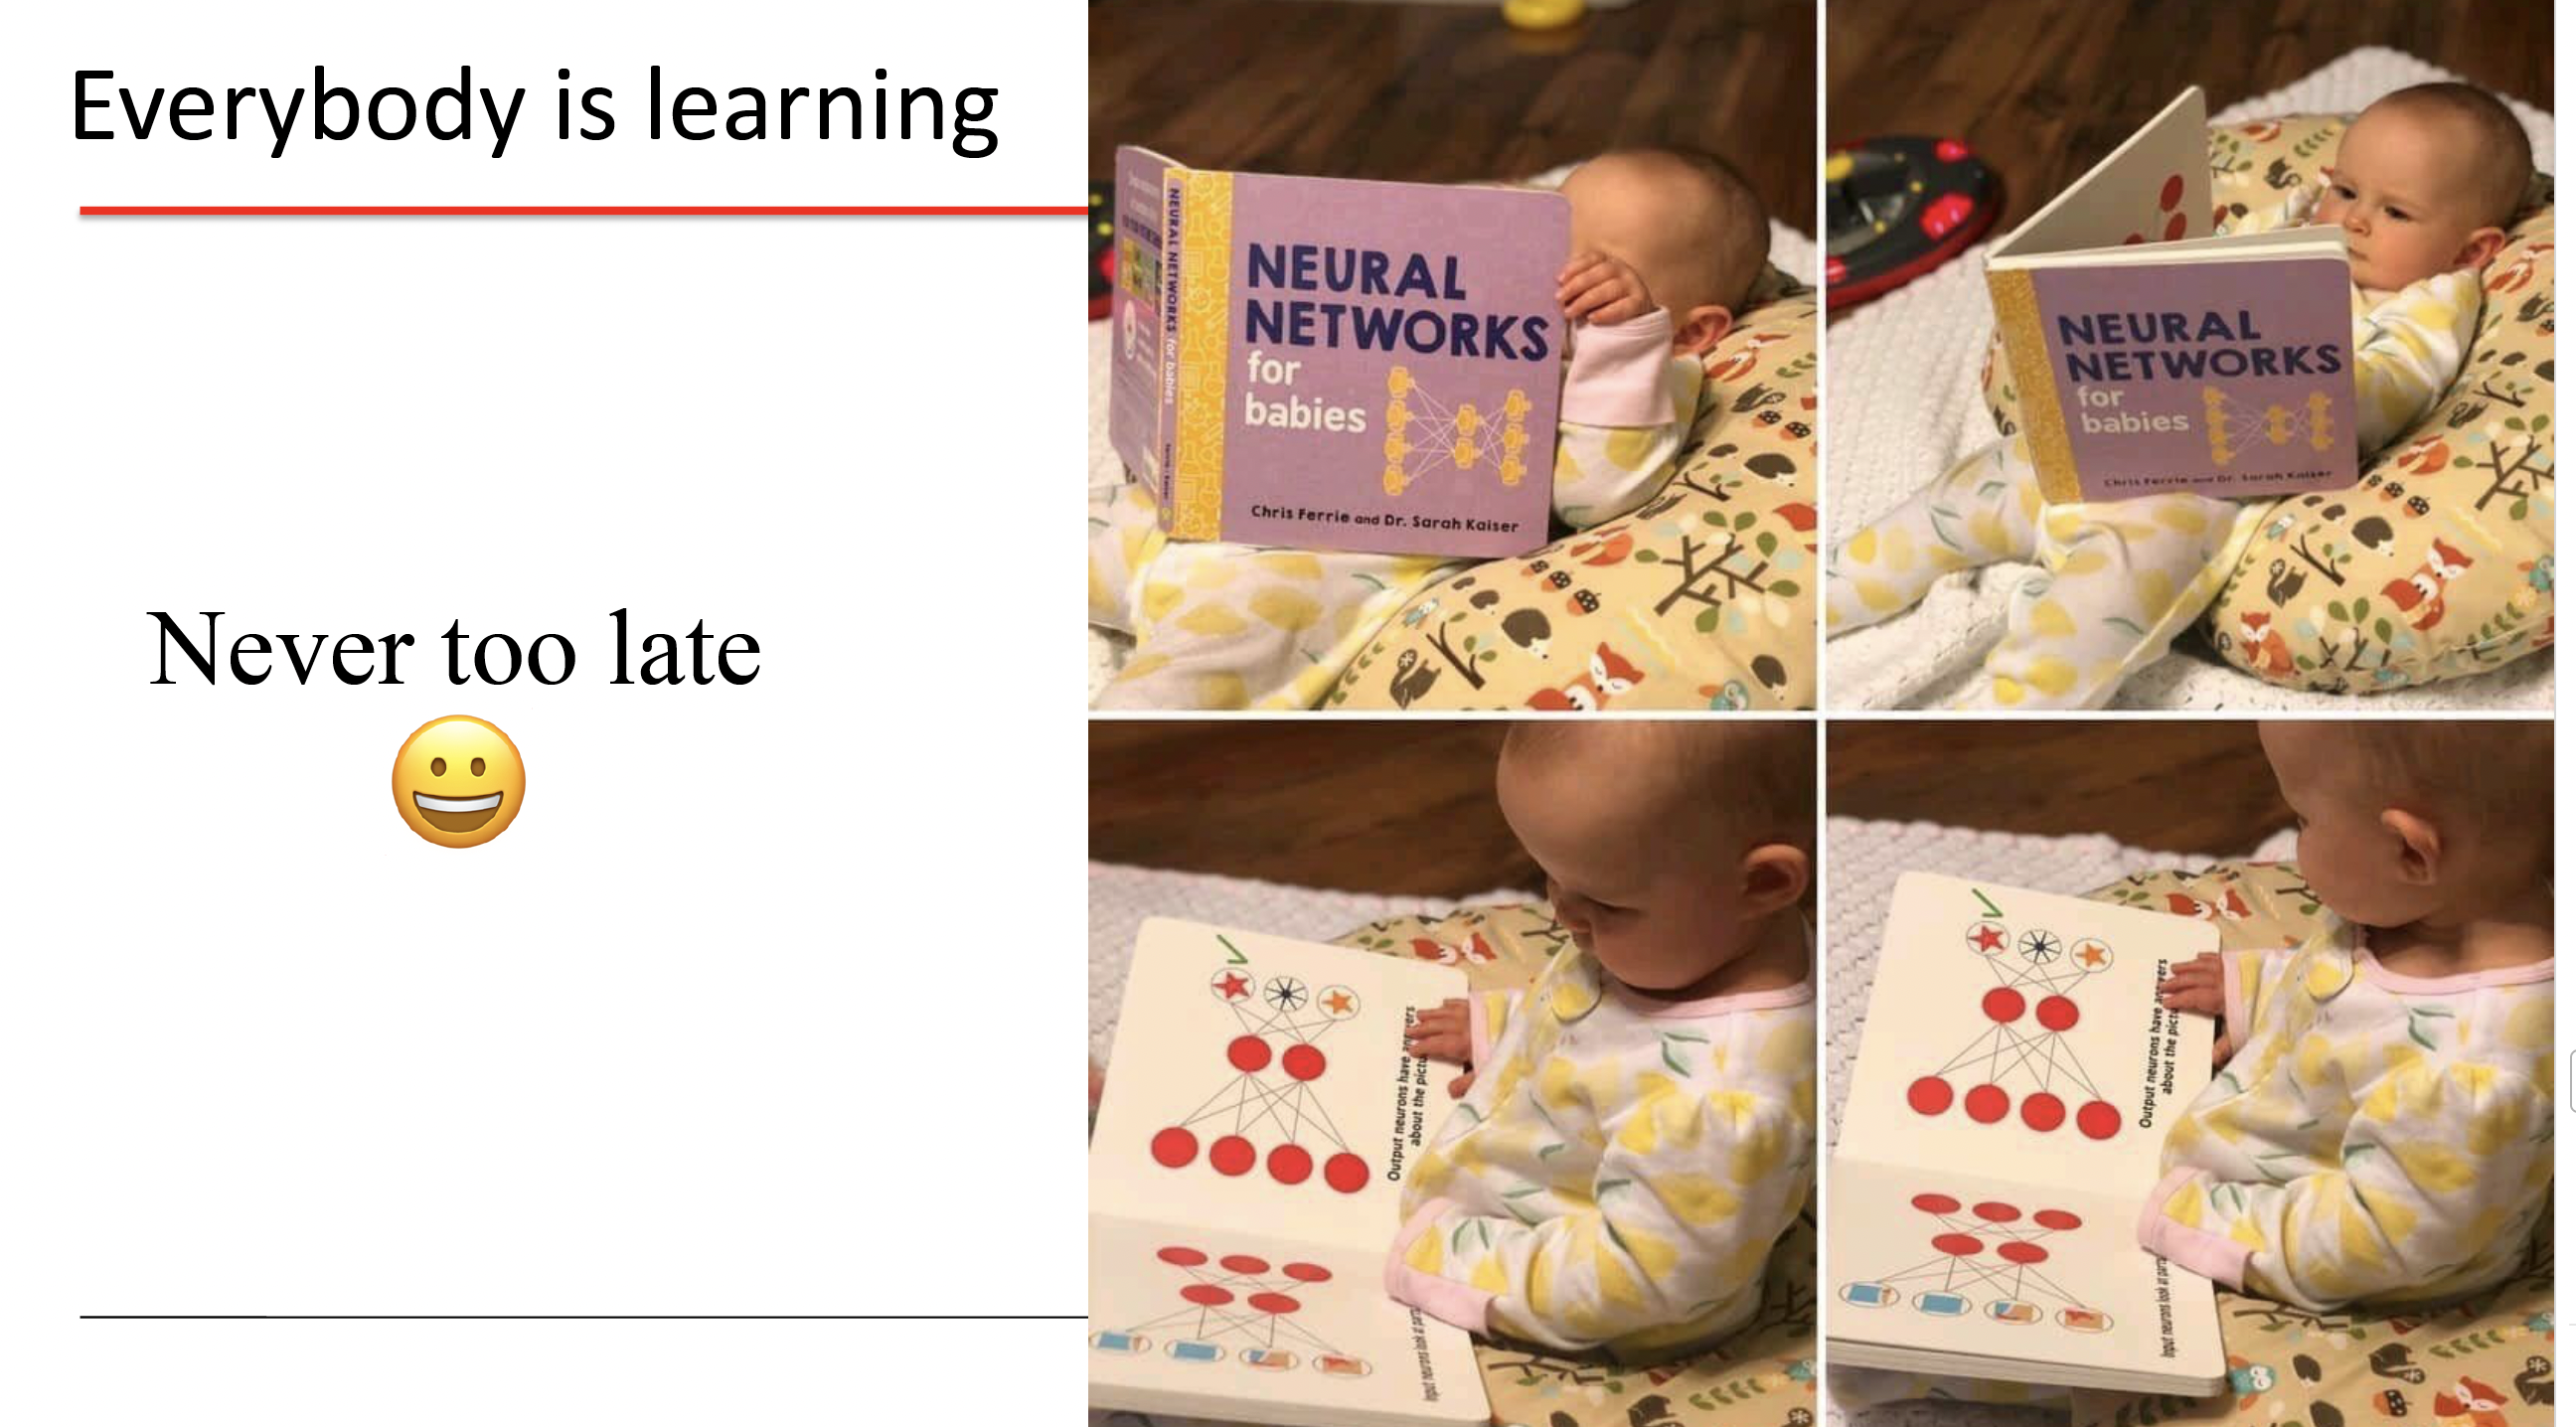
\includegraphics[width=1\linewidth]{figures/Everyone_learningNN}\footnote{CS 229: Prof. Xiangliang Zhang (KAUST)}
\end{figure}
\end{frame}

{
\subsection{Intro to Neural Networks}

\begin{frame}{What is a Neural Network?}
\setbeamercovered{transparent}
 \begin{itemize}[<+->]
    \item A \textbf{Neural Network} is a computational model inspired by the way biological neural networks in the human brain process information.
    \item It consists of \textbf{layers} of interconnected \textbf{nodes}, or \textbf{neurons}, which work together to solve complex problems.
     \item Similarly, brain activity occurs when a \textbf{stimulus} enters the system; information is processed through the network via neurons that extract relevant information, and this information is passed to another area.
    \item Neural networks can \textbf{learn} from data through \textbf{training}, making them powerful tools for \textbf{pattern recognition} and \textbf{predictive modeling}.
\end{itemize}
\end{frame}

\begin{frame}{History of NNs}
\begin{figure}
\includegraphics[width=1\linewidth]{figures/NN-history.pdf}\footnote{CS 229: Prof. Xiangliang Zhang (KAUST)}
\end{figure}
\end{frame}

\begin{frame}{Components of Neural Networks}
\begin{itemize}
    \item Layers
     \item Neurons
    \item Weights
    \item Bias
    \item Activation Functions
    \item Forward Propagation
    \item Loss Function
    \item Backpropagation
    \item Learning Rate
    \item Training Data
    \item Validation and Test Data
\end{itemize}
\end{frame}


\begin{frame}{A Basic Architectures of Neural Networks (1)}
    \begin{itemize}
        \item A neural network consists of several key components:
        \item \textbf{Input Layer:} Each input represents a single predictor variable, which can be a scalar value, a sequence, an image, or even a sequence of images.
        \item \textbf{Output Layer:} For prediction or classification tasks, this layer typically has a single node. For Conditional Density Estimation (CDE), it contains multiple nodes.
        \item \textbf{Hidden Layers:} These layers, often more than one, perform calculations at each node. Each hidden layer's computations are parameterized by weights and biases.
        \item The calculations within a layer can vary in type, including standard, convolutional, and recurrent layers.
        \item The structure of a neural network, referred to as its \textbf{architecture}, defines the arrangement and connectivity of these layers.
    \end{itemize}
\end{frame}

\begin{frame}{A Basic Architectures of Neural Networks (2)}
\begin{figure}
\includegraphics[width=\linewidth]{figures/NNs_pictures}\footnote{\href{https://www.projectpro.io/article/deep-learning-architectures/996}{ProjectPro}}
\end{figure}
\end{frame}

{
\subsection{Components of Neural Networks}
\begin{frame}{Layers}
Neural computing requires a
number of neurons, to be
connected together into a
neural network. Neurons are arranged in
layers. 
    \begin{columns}
        \begin{column}{0.6\textwidth}
           \setbeamercovered{transparent}
 \begin{itemize}[<+->]
                \item \textbf{Input Layer}
                \begin{itemize}
                    \item First layer of neurons.
                    \item Receives raw data directly from the input features.
                \end{itemize}
                \item \textbf{Hidden Layers}
                \begin{itemize}
                    \item Layers between the input and output layers.
                    \item Perform computations.
                    \item Can have one or many hidden layers.
                \end{itemize}
                \item \textbf{Output Layer}
                \begin{itemize}
                    \item Final layer.
                    \item Produces the network's output.
                    \item Structure depends on the specific task (e.g., classification, regression).
                \end{itemize}
            \end{itemize}
        \end{column}
        
        \begin{column}{0.4\textwidth}
            \begin{figure}
                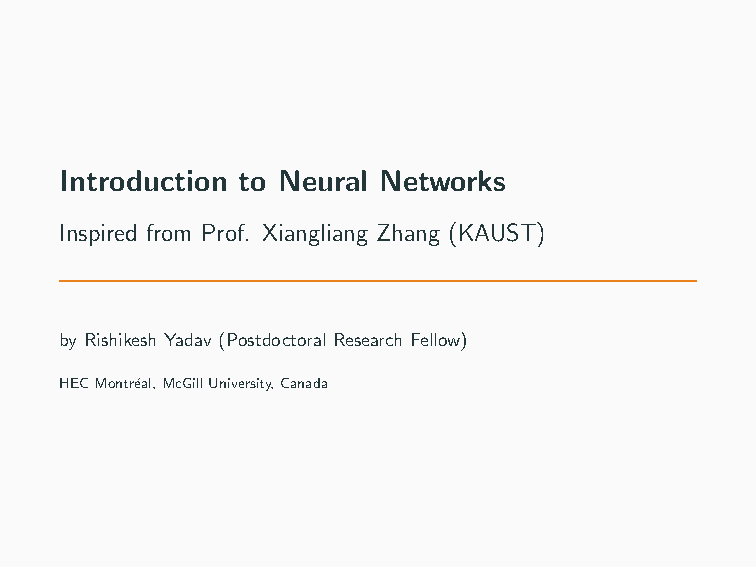
\includegraphics[width=\linewidth]{figures/NNs}\footnote{CS 229: Prof. Xiangliang Zhang (KAUST)}
            \end{figure}
        \end{column}
    \end{columns}
\end{frame}

\begin{frame}{Neurons, Weights, and Biases}
  \setbeamercovered{transparent}
 \begin{itemize}[<+->]
        \item \textbf{Neurons}:
        \begin{itemize}
            \item Basic units of a neural network.
            \item Receive input, process it, and pass it to other neurons.
            \item Apply a mathematical function to generate an output.
        \end{itemize}
        \item \textbf{Weights}:
        \begin{itemize}
            \item Parameters that transform input data within the network.
            \item Each connection between neurons has an associated weight.
        \end{itemize}
        \item \textbf{Biases}:
        \begin{itemize}
            \item Additional parameters in a neuron that allow to fit the data better.
            \item Provide ability to each neuron have output not 0 when inputs are 0.
        \end{itemize}
    \end{itemize}
    \begin{figure}
        \begin{center}
            \includegraphics[width=0.4\linewidth]{figures/neurons.pdf}\footnote{CS 229: Prof. Xiangliang Zhang (KAUST)}
        \end{center}
    \end{figure}
\end{frame}

\begin{frame}{Activation function}
\begin{itemize}
\item The activation function defines the \textbf{output of the node}.  There is two different functions that we can use, but it must satisfy bwlow two properties
\begin{itemize}
\item \textbf{Nonlinear}: If all node has linear activation functions, this is just a linear regression model.
\item \textbf{Continuously differentiable:} Needed for gradient based optimization
\end{itemize}
\end{itemize}
For example, we can think of this activation functions as link function in generalized linear model. In fact a single layered NN is simply a generalized linear model.  
\end{frame}


\begin{frame}{Some Examples of Activation Function }
\begin{figure}
\includegraphics[width=1\linewidth]{figures/activation-functions1.pdf}\footnote{CS 229: Prof. Xiangliang Zhang (KAUST)}
\end{figure}
\begin{figure}
\includegraphics[width=1\linewidth]{figures/activation-functions2.pdf}
\end{figure}
\end{frame}

\begin{frame}{Rectified Linear Unit (ReLu) Activation Function}
\begin{itemize}
\item Older neural networks relied on sigmoid or tanh activation functions that suffsred from vanishing gradient problems which restrict going to deep
\item ReLu\footnote{\url{https://machinelearningmastery.com/rectified-linear-activation-function-for-deep-learning-neural-networks/}} somewhat solve this issue and turn out to be a huge help
\item ReLu has the following forms
\begin{align*}
a(x) =\max\{0, x\}.
\end{align*}
That means
\begin{itemize}
\item The neuron \textbf{activates} only when enough information passes through
\item {\color{red}{One drawbacks}}: Not differentiable at zero.
\end{itemize}
\end{itemize}
\end{frame}
}
{\subsection{Standard Linear and Non-Linear Regressions as Neural Networks}
\begin{frame}{Linear Regression as Neural Networks}
 \begin{figure}
 \includegraphics[width=0.7\linewidth]{figures/NN-LM.pdf}\footnote{CS 229: Prof. Xiangliang Zhang (KAUST)}
 \end{figure}
 \vspace{-1cm}
 $f(\cdot)$
 \begin{itemize}
\item The identity function in the case of regression.
\item A nonlinear activation function in the case of classification.
\end{itemize}
Learning object: 
\begin{itemize}
\item Learn $\bm w$'s so the function fits the data well.
\item The basis functions are fixed functions of $X$.
 \end{itemize}
\end{frame}



\begin{frame}{Non Linear Regression as Neural Networks}
 \begin{figure}
 \includegraphics[width=0.7\linewidth]{figures/NN-NonLM.pdf} \footnote{CS 229: Prof. Xiangliang Zhang (KAUST)}
 \end{figure}
 \begin{itemize}
\item Learning object: Learn $\bm w$ so the function fits the data well
\item The basis functions are fixed functions of $X$ and $\bm w_1$
 \end{itemize}
\end{frame}

\begin{frame}{A Two-Layer Neural Network (1)}
\begin{figure}
\includegraphics[width=0.65\linewidth]{figures/TwoLayers.pdf}
\end{figure}
\begin{itemize}
\item $D$ input variables
\item $M$ hidden neurons 
\item $K$ outputs 
\item Use the two activation function on weights sum on hidden layers and output layers
\end{itemize}
\end{frame}
}

\begin{frame}{A Two-Layer Neural Network (2)}
Construct $M$ linear combinations of the inputs $x_1,\ldots,x_d$
\begin{align*}
a_j = \sum_{i=0}^{D}w_{ji}^{(1)}x_i, \qquad x_0 =1.
\end{align*}
\begin{itemize}
\item $a_j$ are the activations, $j=1,\ldots,M$.
\item $w_{ji}^{(1)}$ are the layer one weights, $i=1,\ldots,D$.
\item $w_{j0}^{(1)}$ are the layer one biases.
\end{itemize}
Each linear combination $a_j$ is transformed by a (non-linear differentiable) activation function
\begin{align*}
z_j = h(a_j).
\end{align*} 
\end{frame}


\begin{frame}{A Two-Layer Neural Network (3)}
The hidden output $z_j = h(a_j)$ are linearly combined in layer two:
\begin{align*}
a_k = \sum_{j=0}^{M}w_{kj}^{(2)}z_j, \qquad z_0 =1.
\end{align*}
\begin{itemize}
\item $a_k$ are the output activations, $k=1,\ldots,K$.
\item $w_{kj}^{(2)}$ are the layer two weights, $j=1,\ldots,M$.
\item $w_{k0}^{(2)}$ are the layer one biases. 
\end{itemize}
The output activations $a_k$ are transformed by the output (non-linear differentiable) activation function
\begin{align*}
y_k = \sigma(a_k).
\end{align*} 
\begin{itemize}
\item $y_k$ are the final outputs.
\item $\sigma(\cdot)$ is like $h(\cdot)$, but often sigmoid function for classification and linear function for Regressions.
\end{itemize}
\end{frame}

\begin{frame}{A Two-Layer Neural Network (4)}
After substituting $y_k = \sigma(a_k)$ the definitions of $a_j$ and $a_k:$
\begin{align*}
y_k(\bm x, \bm w) = \sigma\left(\sum_{i=0}^{M} w_{kj}^{(2)} h\left(\sum_{i=0}^{D} w_{ji}^{(1)} x_i \right) \right).
\end{align*}
Evaluation of this is called \textbf{forward propagation}.
\begin{itemize}
\item $h(\cdot)$ and $\sigma(\cdot)$ are a sigmoid functions, e.g.,  the logistics function.
\begin{align*}
s(a) = \frac{1}{1+ \exp(-a)}, \quad s(a) \in [0,1].
\end{align*}
\item If $\sigma(a)$ is the identity, then a regression model is obtained.
\end{itemize}
\end{frame}



\begin{frame}{Properties \& Generalizations}
\begin{itemize}
    \item Typically, \( K < D < M \). If \( M < D \) or \( M < K \), information may be lost at the hidden units.
    \item A multilayer network of linear units (where all \( h(\cdot) \) are linear) is not interesting and can be simplified to a network without hidden units.
    \item There may be more than one layer of hidden units.
    \item Individual units need not be fully connected to the next layer.
    \item Individual links may skip over one or more subsequent layers.
    \item There may be symmetries in the weight space, meaning that different choices of \( w \) may define the same mapping from input to output.
\end{itemize}
\end{frame}

{\subsection{Training}

\begin{frame}{Learning the Weights}
\begin{itemize}
    \item The learning rule modifies the weights according to the input patterns that it is presented with.
    \item In a sense, artificial neural networks (ANNs) learn by examples, similar to their biological counterparts.
    \item When the desired outputs are known, the process is referred to as supervised learning.
    \item Each weight will be changed proportional to the error gradient.
\end{itemize}
\end{frame}

\begin{frame}{Error (Loss) Function}
  Training a neural network involves estimating the weights and biases by optimizing a loss function. Let \( N \) represent the number of observations of the response \( t_1, t_2, \ldots, t_N \), and let the neural network predict some output \( \hat{y}_1, \hat{y}_2, \ldots, \hat{y}_N \) (which could be a vector). We express the loss function as \( l(y, \hat{y}) \).
\begin{itemize}
\item {\color{purple}{Regression:}} {\color{red}{Sum of squared}} 
\begin{align*}
E(\bm w) = \frac{1}{2} \sum_{n=1}^{N} \left\{y(\bm x_n, \bm w)- t_n\right\}^2,
\end{align*}
where $t_n, n=1,\ldots,N$ is the observed response. $N$ is the total number if training samples (examples).
\item {\color{purple}{Binary classification:}} NNs with only one output node whose activation function is a logistic sigmoid {\color{red}{Cross-entropy error function}} 
\begin{align*}
E(\bm w) = -\frac{1}{2} \sum_{n=1}^{N} \left\{ t_n\log y(\bm x_n, \bm w) + (1-t_n) \log(1 - y(\bm x_n, \bm w)) \right\}. 
\end{align*}
\end{itemize}
\end{frame}


\begin{frame}{Gradients of Error Function}

\begin{columns}
        \begin{column}{0.6\textwidth}
\begin{itemize}
    \item $y(\bm x_n, \bm w)$ is non-linear w.r.t $\bm w$
    \item Error function $E(\bm w)$ is non-convex
    \item Gradient of $E(\bm w)$, $\nabla E(\bm w)$
    \begin{itemize}
        \item Direction of greatest rate of increase
        \item Minima, $E(\bm w) = 0$
        \item No analytical solution
    \end{itemize}
    \item Gradient descent: Moving through weight space in direction of $-\nabla E(\bm w)$
    \begin{align*}
        \bm w^{\tau +1} = \bm w^{\tau} - \eta \nabla E(\bm w^{\tau}).
    \end{align*}
\end{itemize}
\end{column}
 \begin{column}{0.4\textwidth}
\begin{figure}
    \includegraphics[width=\linewidth]{figures/GlobalMinima}
    \caption{Gradient Descent towards Global Minima}
\end{figure}
\end{column}
\end{columns}
\textbf{Learning by gradients decent algorithm:} Require the evaluation of gradients wrt weight parameters.
\end{frame}


\begin{frame}{How to Evaluate the Gradient}
Need an efficient techniques for {\color{violet}{evaluating the gradient $\nabla E$}}
\begin{align*}
{\color{red}{\text{Back Propogation Algorithm}}}
\end{align*}
Each iteration of the gradient decent algorithm has two stages:
\begin{itemize}
\item Evaluate derivatives of error w.r.t. weights
\item Use derivatives to compute adjustments of the weights 
\end{itemize}
\end{frame}

\begin{frame}{Back Propagating}
\begin{itemize}
\item For output units
\begin{align*}
\delta_k = y(\bm x_n, \bm w) - t_k.
\end{align*}
\item For hidden units 
\begin{align*}
\delta_j = \frac{\partial E}{\partial a_j} = \sum_{k}  \frac{\partial E}{\partial a_k} \frac{\partial a_k}{\partial a_j} = h'\left(a_j\right) \sum_{k} w_{kj} \delta_k.
\end{align*}
\end{itemize}
Summary
\begin{itemize}
\item Apply input $x$, and forward propagate to find the hidden and output activations. 
\item Evaluate $\delta_k$ directly for the outputs units
\item Back propagate $\delta$'s to obtain a $\delta_j$'s for each hidden unit.
\item Evaluate the derivatives  $\frac{\partial E}{\partial a_j} = \delta_i Z_i$
\item  Sum these derivatives to over training cases to compute $\frac{\partial E}{\partial w_{ij}} $  
\end{itemize}
\end{frame}
}

\begin{frame}{Example: Classification Using two-Layer Neural Networks (1)}
\begin{figure}
\includegraphics[width=0.85\linewidth]{figures/classification_examples.pdf}
\end{figure}
\end{frame}


\begin{frame}{Example: Classification Using two-Layer Neural Networks (2)}
\begin{figure}
\includegraphics[width=1\linewidth]{figures/classification_examples_resulst.pdf}
\end{figure}
\end{frame}


\begin{frame}{Learning Issue}
\begin{itemize}
\item  Vanishing gradient problems due to propagated error coming from the other neurons and layers
\begin{itemize}
\item Use of smart activation functions solve this issue 
\end{itemize}
\item Overfitting due to a lot number of hidden units the number of hidden units determines the complexity of the learned function (the number of parameters $\bm w$)
\begin{itemize}
\item 
\item We may allow regularizations 
\item Drop of techniques 
\item Sparse neural networks 
\end{itemize} 
\end{itemize}
\end{frame}


\begin{frame}{Practical Rule of Thumb on deciding hidden units}
\begin{itemize}
\item There is no theoretical results that determines the  minimum number of hidden units.
\item Practical rule of thumb 
\begin{itemize}
\item For binary data $M=2D$
\item For real data $M>>2D$ 
\end{itemize}
\item Multiple hidden layers with fewer nodes maybe trained faster for similar quality in some applications 
\end{itemize}
\end{frame}

}

%{
%\section{Introduction to R-Keras}{
%\subsection{Settings and installation}
%\begin{frame}{Settings and installation}
%\begin{itemize}
%    \item First thing’s first, let’s get Keras installed:
%    \begin{enumerate}
%        \item Open \texttt{installation.R}.
%        \item Download and install Python 3.8.4 from \url{https://www.python.org/downloads/macos/} (unless you already have a working version of Python 3.5).
%        \item Install the \texttt{keras} and \texttt{tensorflow} R packages.
%        \item Create a virtual Python environment.
%        \item Configure the RStudio Python interpreter (you will need to restart the R session for this).
%        \item Install the latest versions of the Python libraries \texttt{tensorflow} and \texttt{keras}.
%        \item Don’t touch any Python2 installations!
%    \end{enumerate}
%\end{itemize}
%
%\end{frame}
%
%
%\begin{frame}{What is Keras?}
%\begin{itemize}
%    \item Keras is a high-level API for fast deep learning, developed by Google and primarily written in Python. It was released in 2015.
%    \item Initially, Keras supported multiple back-ends (Theano, MILA; CNTK by Microsoft). However, it now exclusively runs on top of TensorFlow.
%    \item TensorFlow is a free, open-source machine learning library (not limited to deep learning). It is written in Python, C++, and CUDA (for GPU support), handling all the lower-level computations for Keras.
%    \item Keras is the most widely used deep learning software due to its simple yet powerful framework, followed closely by Facebook’s PyTorch. PyTorch can also be used in R (see \href{https://www.rstudio.com/blog/torch/}{Torch in R}).
%\end{itemize}
%\end{frame}
%
%}
%{
%\subsection{Conditional density estimation}
%\begin{frame}{Conditional density estimation?}
%\begin{itemize}
%    \item Let \( Y \) be a response variable with covariates/predictors \( X \):
%    \begin{itemize}
%        \item Conditional density estimation is a generalization of normal (mean/least-squares) regression.
%        \item In mean regression, we model \( \mathbb{E}[Y \mid X] \) as a function \( m \) of predictors.
%        \item For cumulative distribution functions (CDF), we model the entire conditional density \( f(Y \mid X) \).
%        \item In a parametric framework, we let \( Y \mid X \sim F(\cdot) \) for a parameter set \( \theta \) and then let \( \theta \) be a function \( m \) of observations \( x \) of \( X \).
%        \item Applications include:
%        \begin{itemize}
%            \item Prediction and Gaussian density estimation (with fixed \( \theta = 1 \)).
%            \item Classification problems and multinomial density estimation.
%        \end{itemize}
%        \item We are going to estimate \( m(x) \) using Deep Learning.
%    \end{itemize}
%\end{itemize}
%\end{frame}
%}
%
%}

\end{document}
